Comparisons of the neutrino selection between data and Monte Carlo simulation only gain meaning within the context of properly characterized uncertainties on both the data measurement and the Monte Carlo simulation. The data measurement inherently contains statistical uncertainty reflecting the size of the data set. The expectation from the Monte Carlo simulation has, in addition to statistical uncertainty, other sources of systematic uncertainty arising from the uncertainty in the BNB flux, the neutrino interaction model, and the response of the detector to neutrino interactions.

The covariance matrix formalism \cite{Eaton2007} is used to accurately capture the scale and bin-to-bin correlations of each source of uncertainty. Under the assumption that the underlying sources of uncertainty are independent, the bilinearity of the covariance matrix allows for the independent calculation of covariance matrices for each source and the calculation of the total covariance matrix as the sum over all covariance matrices. It is worth noting that the effect of the sources of uncertainty are in general correlated to some degree, but the underlying sources are often independent. Section \ref{sec:bnb_flux} describes the estimation of uncertainties associated with the BNB flux prediction. Section \ref{sec:xsec} describes the estimation of uncertainties associated with the modeling of $\nu$-Ar interactions using the GENIE event generator. Section \ref{sec:detector_response} describes the procedure for estimating systematic uncertainties associated with the modeling of detector effects. Finally, a summary of the overall uncertainties in the analysis is presented in Section \ref{sec:uncertainty_conclusion}.

\subsection{BNB Flux Uncertainties}
\label{sec:bnb_flux}
The BNB flux prediction used for ICARUS is based on the flux prediction computed for MiniBooNE \cite{Aguilar2009}. The production rate of hadrons through $p$-Be interactions in the target is modeled using a GEANT4 simulation \cite{Agostinelli2003} and includes some additional re-weighting of pion production based on hadron production data as measured in the HARP experiment \cite{Prior2005}. In addition to the uncertainties arising from hadron production, there are also uncertainties associated with the re-scattering of pions and protons in the beryllium and aluminum horn through quasielastic and inelastic processes and the mis-modeling of current flow through the magnetic focusing horn. Additionally, there is a flat 2\% uncertainty associated with the total number of POT due to the uncertainty in the measured POT from the BNB \cite{Aguilar2009}.

The estimation of the flux covariance matrix follows a ``many-universe'' technique, where the flux parameters associated with these systematic uncertainty sources are varied following a Gaussian distribution centered at the predicted central value and width. A total of $M=1000$ universes are simulated in this way for each systematic parameter and each neutrino interaction is assigned a weight reflecting the probability of the true parameter living in that universe. After binning the selected interactions for each universe, the covariance $E_{ij}^\alpha$ between bins $i$ and $j$ under the effect of systematic parameter $\alpha$ is computed as:

\begin{equation}
    \label{eq:covariance}
    E_{ij}^{\alpha} = \frac{1}{M} \sum_{m=1}^M (N_{CV}^i - N_{\alpha, m}^i)(N_{CV}^j - N_{\alpha, m}^j)
\end{equation}

\noindent
where $N_{CV}^i$ is the central value prediction for bin $i$ and $N_{\alpha,m}^i$ is the content of bin $i$ in the universe $m$. The total covariance matrix is then computed as the sum of the covariance matrices for each systematic parameter. This process is then be repeated for each reconstructed variable discussed in Section \ref{sec:variables_of_interest}. A breakdown of the flux uncertainty is shown in Table \ref{tab:flux}.

\begin{table}
    \centering
    \caption{A breakdown of the overall scale of each flux uncertainty for each of the three signal definitions. Beamline uncertainties are those associated with the re-scattering of hadrons in the target and the modeling of the magnetic focusing horn. Hadron production uncertainties are those associated with the production of hadrons in the target.}
    \begin{tabular}{ccccc}
\toprule
Uncertainty & Type & $1\mu1p$ [\%] & $1\mu Np$ [\%] & $\nu_\mu$ CC [\%] \\
\midrule
Skin Depth & Beamline & 2.2 & 2.7 & 3.2 \\
Horn Current & Beamline & 0.4 & 0.5 & 0.5 \\
$\pi^+$ & Hadron Production & 4.7 & 4.7 & 4.8 \\
$\pi^-$ & Hadron Production & 0.1 & 0.0 & 0.1 \\
$K^+$ & Hadron Production & 0.1 & 0.1 & 0.2 \\
$K^-$ & Hadron Production & 0.0 & 0.0 & 0.0 \\
$K^0_L$ & Hadron Production & 0.0 & 0.0 & 0.0 \\
Nucleon Inelastic & Beamline & 0.9 & 0.9 & 0.9 \\
Nucleon QE & Beamline & 2.5 & 2.5 & 2.5 \\
Nucleon Total & Beamline & 0.8 & 0.8 & 0.8 \\
$\pi$ Inelastic & Beamline & 1.2 & 1.2 & 1.2 \\
$\pi$ QE & Beamline & 0.8 & 0.9 & 0.8 \\
$\pi$ Total & Beamline & 0.7 & 0.8 & 0.8 \\
POT & Beamline & 2.0 & 2.0 & 2.0 \\
\midrule
Total Flux &  & 6.7 & 6.9 & 7.3 \\
\bottomrule
\end{tabular}
    \label{tab:flux} 
\end{table}

\subsection{Neutrino Interaction Uncertainties}
\label{sec:xsec}

Neutrino interactions are simulated using the GENIE event generator \cite{Andreopoulos2015} for the central value prediction. Within GENIE, there are a large number of parameters available for re-weighting that are used in the simulation of neutrino interactions. To estimate the uncertainty in the neutrino interaction model, the many-universe technique is used to vary these parameters in order to individually characterize their effect on the downstream analysis. The covariance matrix for each parameter is computed with Equation \ref{eq:covariance} as done for the flux uncertainties. The total covariance matrix is then computed as the sum of the covariance matrices for each parameter. A breakdown of the neutrino interaction model uncertainty is shown in Table \ref{tab:xsec}.

\begin{table}
    \centering
    \caption{A breakdown of the overall scale of each neutrino interaction model uncertainty for each of the three signal definitions.}
    \resizebox{0.99\textwidth}{!}{\begin{tabular}{ccccc}
\toprule
Uncertainty & Description & $1\mu1p$ [\%] & $1\mu Np$ [\%] & $\nu_\mu$ CC [\%] \\
\midrule
ZExpAVariationResponse & Z-expansion description of the axial-vector form factor on CC-QE & 9.6 & 8.1 & 6.3 \\
RPA CCQE & RPA suppression of CC-QE & 4.7 & 3.3 & 6.8 \\
Coulomb CCQE & The strength of the electromagnetic potential for the Coulomb corrections on CC-QE & 0.5 & 0.4 & 0.3 \\
Norm CCMEC & Normalization of CC-MEC & 7.5 & 10.2 & 7.1 \\
Norm NCMEC & Normalization of NC-MEC & 0.0 & 0.0 & 0.0 \\
NCEL Variation Response & Variation of the dipole form factor on NCEL & 0.1 & 0.1 & 0.1 \\
CCRES Variation Response & Variation of the dipole form factor on CC-RES & 2.2 & 4.5 & 6.7 \\
NCRES Variation Response & Variation of the dipole form factor on NC-RES & 0.4 & 0.4 & 0.5 \\
NonRESBGvpCC1pi & Scale factor for the non-resonant background level of $\nu$-p CC + 1$\pi$ & 0.0 & 0.1 & 0.1 \\
NonRESBGvpCC2pi & Scale factor for the non-resonant background level of $\nu$-p CC + 2$\pi$ & 0.1 & 0.2 & 0.6 \\
NonRESBGvpNC1pi & Scale factor for the non-resonant background level of $\nu$-p NC + 1$\pi$ & 0.0 & 0.0 & 0.0 \\
NonRESBGvpNC2pi & Scale factor for the non-resonant background level of $\nu$-p NC + 2$\pi$ & 0.0 & 0.0 & 0.1 \\
NonRESBGvnCC1pi & Scale factor for the non-resonant background level of $\nu$-n CC + 1$\pi$ & 0.1 & 0.2 & 0.4 \\
NonRESBGvnCC2pi & Scale factor for the non-resonant background level of $\nu$-n CC + 2$\pi$ & 0.1 & 0.2 & 0.7 \\
NonRESBGvnNC1pi & Scale factor for the non-resonant background level of $\nu$-n NC + 1$\pi$ & 0.2 & 0.2 & 0.2 \\
NonRESBGvnNC2pi & Scale factor for the non-resonant background level of $\nu$-n NC + 2$\pi$ & 0.0 & 0.0 & 0.0 \\
NonRESBGvbarpCC1pi & Scale factor for the non-resonant background level of $\bar{\nu}$-p CC + 1$\pi$ & 0.0 & 0.0 & 0.0 \\
NonRESBGvbarpCC2pi & Scale factor for the non-resonant background level of $\bar{\nu}$-p CC + 2$\pi$ & 0.0 & 0.0 & 0.0 \\
NonRESBGvbarpNC1pi & Scale factor for the non-resonant background level of $\bar{\nu}$-p NC + 1$\pi$ & 0.0 & 0.0 & 0.0 \\
NonRESBGvbarpNC2pi & Scale factor for the non-resonant background level of $\bar{\nu}$-p NC + 2$\pi$ & 0.0 & 0.0 & 0.0 \\
NonRESBGvbarnCC1pi & Scale factor for the non-resonant background level of $\bar{\nu}$-n CC + 1$\pi$ & 0.0 & 0.0 & 0.0 \\
NonRESBGvbarnCC2pi & Scale factor for the non-resonant background level of $\bar{\nu}$-n CC + 2$\pi$ & 0.0 & 0.0 & 0.0 \\
NonRESBGvbarnNC1pi & Scale factor for the non-resonant background level of $\bar{\nu}$-n NC + 1$\pi$ & 0.0 & 0.0 & 0.0 \\
NonRESBGvbarnNC2pi & Scale factor for the non-resonant background level of $\bar{\nu}$-n NC + 2$\pi$ & 0.0 & 0.0 & 0.0 \\
RDecBR1gamma & Scale factor for the branching fraction of X + 1$\gamma$ & 0.0 & 0.0 & 0.0 \\
RDecBR1eta & Scale factor for the branching fraction of X + 1$\eta$ & 0.2 & 0.3 & 0.4 \\
COH Variation Response & Normalization of the Coherent production process & 0.1 & 0.1 & 0.2 \\
DISBY Variation Response & Normalization of the BY model of the DIS process & 0.0 & 0.0 & 0.0 \\
FSI $\pi$ Variation Response & Variation for FSI involving pions & 1.2 & 3.5 & 0.7 \\
FSI N Variation Response & Variation for FSI involving nucleons & 3.9 & 3.0 & 1.2 \\
\midrule
Total Cross Section &  & 14.7 & 15.7 & 14.6 \\
\bottomrule
\end{tabular}}
    \label{tab:xsec}
\end{table}

Many of these individual parameters have a small effect on the overall uncertainty, but there are a few worth highlighting:

\begin{itemize}
    \item The parameter associated with the Z-expansion of the axial form factor has a large effect on the overall uncertainty. This is especially true for the two exclusive channels, which are more dominated by QE interaction modes.
    \item The RPA suppression parameter has an effect in the range of 3-7\%. This is largest for the inclusive channel.
    \item The normalization for CC MEC processes is large for all channels, but is especially large for the 1$\mu$N$p$ channel. This is due to the larger contribution of MEC processes to the 1$\mu$N$p$ channel.
    \item The parameter controlling the dipole form factor for CC resonant production is progressively larger as the final state becomes less restrictive due to higher contributions from resonant production.
    \item Many of the parameters associated with anti-neutrino interactions have vanishingly small effects on the overall uncertainty. This is due to the low flux of anti-neutrinos in the BNB in the ``neutrino-mode'' horn configuration, which has been the operating mode for all physics datasets collected by the ICARUS detector.
\end{itemize}

Overall, all three channels have a resulting total uncertainty due to interaction model uncertainties of around 15\%. The 1$\mu$N$p$ channel has a slightly larger uncertainty (around 1\% more) due to the larger contribution of MEC processes to this channel, which have larger uncertainties associated with them.

\subsection{Detector Response Uncertainties}
\label{sec:detector_response}
The detector response uncertainty reflects many non-idealizations of the ICARUS detector and the underlying detector physics that can impact event reconstruction and signal selection. The effects considered can be broadly grouped into three categories:

\begin{enumerate}
    \item Light yield, scintillation photon propagation, and optical response throughout the detector.
    \item Electron-ion recombination, space charge effects, electron lifetime, diffusion, and other processes affecting drifting ionization charge.
    \item Variable TPC channel gain, non-uniformities in response across the wire planes, electronic noise, and other effects impacting signal reconstruction associated with the TPC wires.
\end{enumerate}

The detector response uncertainty is characterized through dedicated detector variation samples. Each detector variation sample implements a single variation in some underlying component of the Monte Carlo simulation that fully covers some aspect of the detector response that is not fully understood or known to be insufficiently modeled. 

A sample of $N_{CV}$ total events generated with the nominal simulation parameters and run through the full detector simulation and event reconstruction is used as the central value prediction. The same set of $N_{CV}$ events is then run through the full detector simulation and event reconstruction with the detector variation applied. Random processes in the GEANT4 simulation of particle trajectories and secondaries may produce additional statistical differences between the nominal and systematic variation sample, so a workflow which shares the generated particles and their trajectories between both samples is used to characterize the detector systematics. A diagram representing the full simulation chain for both the nominal simulation and a detector variation sample is shown in Figure \ref{fig:systematic_variation_sample_flow}.

\begin{figure}
    \centering
    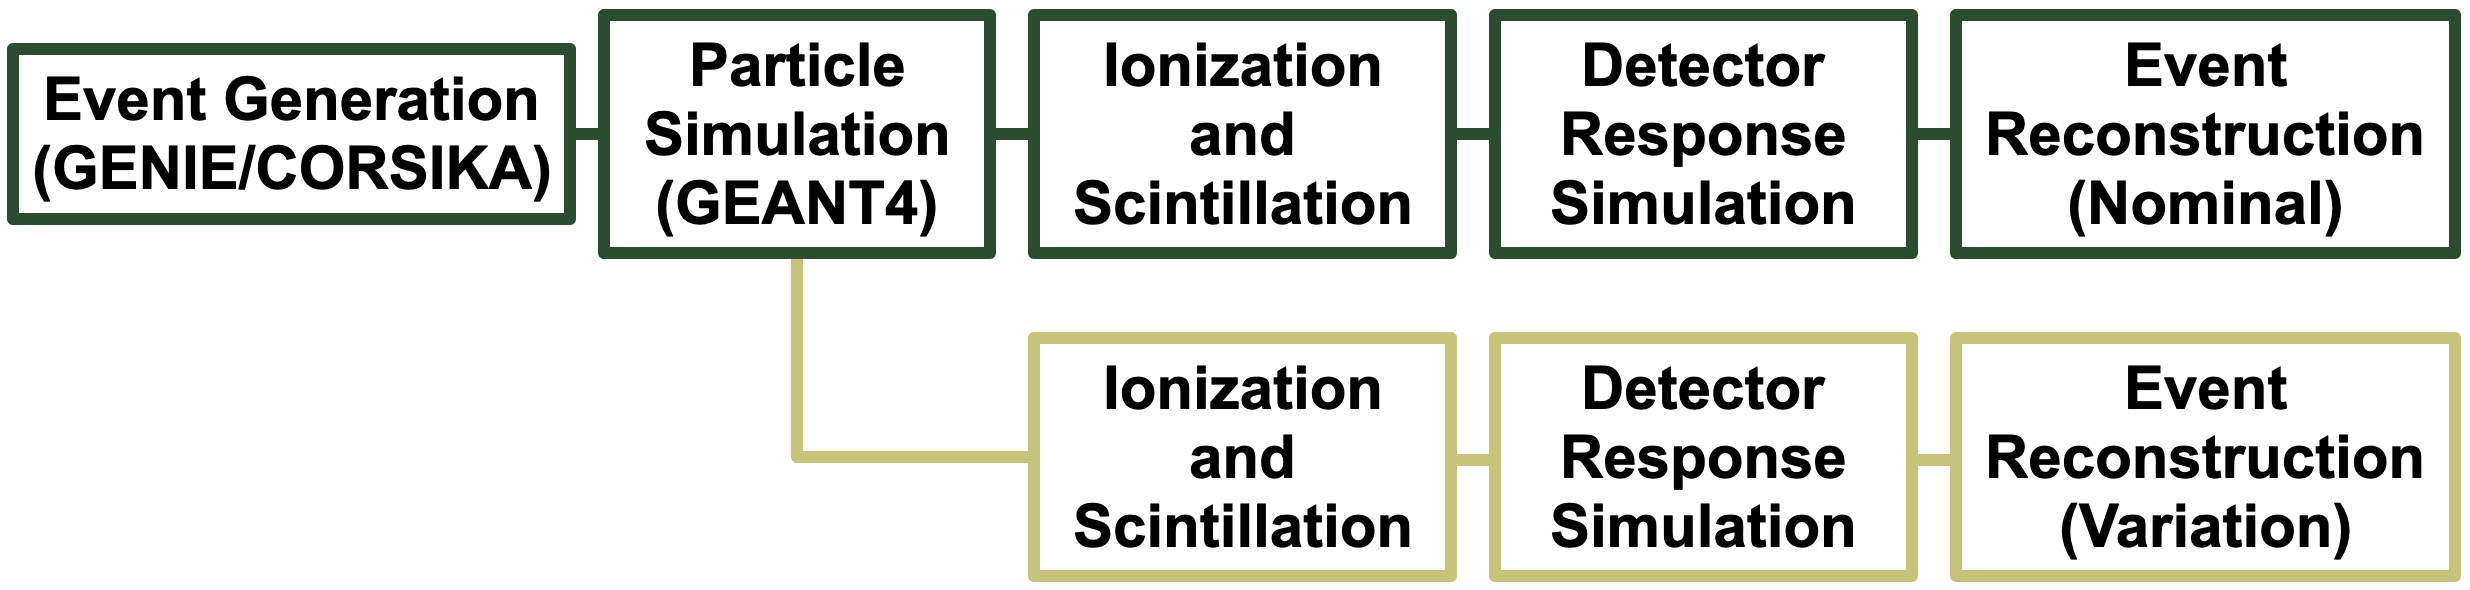
\includegraphics[width=0.95\textwidth]{figures/systematics/systematic_variation_sample_flow.png}
    \caption{A diagram representing the full simulation chain for both the nominal simulation (green) and a detector variation sample (gold). The samples share the same set of generated events including particle trajectories and daughters, but downstream processes may vary according to statistical processes or the variation itself.}
    \label{fig:systematic_variation_sample_flow}
\end{figure}

For this analysis, samples of $N_{CV} = 200,000$ events were generated for the central value and each detector variation sample. The choice of detector systematics to vary was made based on the expected impact of the variation on the final event selection. This list is not exhaustive and further detector systematics will be studied in the future. Due to the large time and computational resources required to generate each sample, the decision was made to use neutrino-only samples to characterize the detector systematics. Though the presence of cosmic rays does have an impact on the selection, the relative effect of the variation on the selection is expected to be similar between the neutrino-only and full samples. The detector variation samples produced for this analysis are:

\paragraph{TPC Signal Shape:}
This is a variation in the shape of the signal response on the wire planes. The central value sample uses a signal response that was tuned with cosmic muon data, whereas the variation sample uses the original signal response that was produced with a simulation. This is a conservative estimate of the uncertainty in the signal shape, as this is essentially treating the full effect of a known bias as a systematic uncertainty. Future detector systematic studies within ICARUS will aim to better characterize the uncertainty in the signal shape.

\paragraph{First Induction Plane Gain:}
This is a variation in the gain of the first induction plane of $\pm 15\%$, implemented separately as two distinct samples. These variations reflect the un-simulated variation of the gain across the first induction plane.

\paragraph{PMT Quantum Efficiency:}
There is a known data to simulation discrepancy in the optical model that is in the process of being understood. This variation is meant to cover this discrepancy by varying the quantum efficiency of the PMTs by $4\%$. In addition to potential impacts on the flash matching performance, this variation also directly impacts the emulated trigger decision and therefore may cause a shift in the selected events by changing the trigger efficiency.

\paragraph{TPC Coherent Noise:}
The coherent component of the TPC noise varied by $4.9\%$ with respect to the nominal noise model over the duration of Run 2. A positive variation of this scale is applied to the nominal simulation to cover this discrepancy.

\paragraph{TPC Intrinsic Noise:}
Similar to the coherent noise variation, the intrinsic noise of the TPC varied by $3.7\%$ with respect to the nominal noise model over the duration of Run 2. A positive variation of this scale is applied to the nominal simulation to cover this discrepancy.

\paragraph{Electron-ion Recombination:}
The recombination model used in the nominal simulation is the Modified Box model, as measured by ArgoNeuT \cite{Acciarri2013}. Recently, the dependence of recombination on the angle of the track with respect to the electric field has been measured at ICARUS and encapsulated in a model referred to as the ``Ellipsoidal'' recombination model. The variation sample uses this model to estimate the uncertainty that may arise from improperly modeling recombination.

\vspace{\baselineskip}
The comparison of the central value and variation samples is used to estimate the uncertainty in the detector response. The procedure used is covered in the following section.

\subsubsection{Bootstrapping}
\label{sec:bootstrapping}

The detector response uncertainty is estimated using a bootstrapping technique similar to the one employed in several differential cross section measurements performed by the MicroBooNE collaboration \cite{Abratenko2022f,Abratenko2022e,Abratenko2024}. An overview of bootstrapping techniques can be found in \cite{Chernick2011}. The general idea is to estimate the uncertainty in a measurement by repeatedly sampling the data with replacement and computing the quantity of interest for each sample. The distribution of these quantities is then used to estimate the uncertainty in the measurement. This method inherently captures the bin-to-bin correlations in the uncertainty, which is important for the downstream analysis. The assumption made in this method is that the distribution being sampled from is sufficiently large enough to represent the true distribution of the data.

In the bootstrapping technique used for this analysis, the set of common events between the central value and a variation sample is sampled $N_{CV}$ times with replacement to form one ``universe.'' In each universe, the selected signal candidates from the central value sample and the variation sample are binned according to the reconstructed variable of interest. A difference vector $\vec{V}_{D,i}$ is computed for the $i$'th universe as the difference across the bins between the two samples. This process is repeated $N_{\text{bootstrap}} = 1000$ times to form a distribution of difference vectors. The average $1\sigma$ deviation $\vec{V}^{nominal}_D$ is then computed as the average of the difference vectors across the universes.

The uncertainty on $\vec{V}^{nominal}_D$ is then computed as the covariance matrix $M_R$ of the difference vectors across the universes as is described in Equation \ref{eq:covariance}. This covariance matrix can be understood as the matrix governing the Gaussian distribution of the difference vectors, or in other words the matrix that describes how to perturb $\vec{V}^{nominal}_D$ according to the fluctuations seen in the bootstrapping procedure.

The overall covariance matrix for the variation is then computed using both $\vec{V}^{nominal}_D$ and $M_R$ in a way that fully captures the detector response uncertainty. A new set of universes is generated in this step, with $N_{\text{universes}} = 1000$. In each universe, the matrix $M_R$ is used to generate a perturbation $\delta \vec{V}_D$ by sampling from a Gaussian distribution centered at $\vec{V}^{nominal}_D$ with covariance $M_R$. This is realized by computing the Cholesky decomposition of $M_R$ and using this to generate a random vector with elements correlated according to $M_R$ from a vector with normally distributed, uncorrelated elements. The perturbation $\delta \vec{V}_D$ is then added to the central value vector $\vec{V}^{nominal}$ and scaled by a unit Gaussian $r_i$ to form the final vector $\vec{V}^{final}_D$, as shown in Equation \ref{eq:final_vector}.

\begin{equation}
    \label{eq:final_vector}
    \vec{V}^{final}_{D,i} = r_i \left(\vec{V}^{nominal} + \delta \vec{V}_{D,i}\right)
\end{equation}

\noindent
This set of vectors $\vec{V}^{final}_{D,i}\ \forall i \in [1, N_{\text{universes}}]$ is then used to compute the covariance matrix $M_D$ that describes the uncertainty on the event selection due to the variation in the detector response. This process is then repeated for each of the variation samples and for each of the reconstructed variables discussed in Section \ref{sec:variables_of_interest}. These covariance matrices can then be combined to form the total covariance matrix for the detector response uncertainty. A breakdown of the detector response uncertainty is shown in Table \ref{tab:detector_systematics}

\begin{table}
    \centering
    \caption{A breakdown of the overall scale of each detector response uncertainty for each of the three signal definitions.}
    \begin{tabular}{ccccc}
\toprule
Uncertainty & Type & $1\mu1p$ [\%] & $1\mu Np$ [\%] & $\nu_\mu$ CC [\%] \\
\midrule
TPC Signal Shape & TPC & 5.5 & 6.4 & 3.3 \\
Increased Front Induction Gain & TPC & 2.1 & 2.2 & 2.2 \\
Decreased Front Induction Gain & TPC & 2.3 & 2.2 & 2.4 \\
Ellipsoidal Recombination & TPC & 2.1 & 1.9 & 2.5 \\
Increased Coherent Noise & TPC & 2.1 & 2.2 & 2.2 \\
Increased Intrinsic Noise & TPC & 2.5 & 2.3 & 2.4 \\
PMT Quantum Efficiency & PMT & 2.1 & 2.2 & 2.2 \\
\midrule
Total Detector &  & 8.1 & 8.6 & 6.9 \\
\bottomrule
\end{tabular}
    \label{tab:detector_systematics}
\end{table}

From these results, it is clear that the variation of the TPC signal shape is the most impactful on this analysis. This is not surprising as the signal shape is a fundamental aspect of the signal processing and affects all downstream reconstruction. Additionally, as noted in the summary of the variations above, this variation treats the full effect of a known bias as a systematic uncertainty. Work is ongoing within ICARUS to establish post-calibration uncertainties to more accurately model this effect. In contrast, the other variations have reached a floor of around 2\% uncertainty. A few things are likely contributing to this floor: the statistical nature of the bootstrapping technique, the size of the sample used to estimate the uncertainty, and the remaining statistical processes that are not fully shared between the central value and variation samples. The actual uncertainty due to these variations is likely smaller than the 2\% floor, so the TPC signal shape uncertainty can be treated as lower bound on the uncertainty due to the detector response.

\subsubsection{Summary of Event Selection Uncertainties}
\label{sec:uncertainty_conclusion}

The overall uncertainty in the event selection is computed as the sum of the covariance matrices for each source of uncertainty described in the previous sections. This total covariance matrix can then be used to place uncertainty bars on the histogram entries for each reconstructed variable used in the analysis, thus allowing for a visual representation of the uncertainty in the event selection. A more quantitative use of the covariance matrix is in the calculation of the $\chi^2$ test statistic between data and the prediction. This will be discussed in more detail in the next chapter. A summary of the overall uncertainty in the event selection, broken down by category, is shown in Table \ref{tab:overall_systematics}. The total correlation matrix for the 1$\mu$1$p$, 1$\mu$N$p$, and $\nu_\mu$ CC inclusive channels is shown in Figure \ref{fig:correlation_matrices}.

\begin{table}
    \centering
    \caption{A breakdown of the overall scale of each uncertainty source by category for each of the three signal definitions.}
    \resizebox{0.99\textwidth}{!}{\begin{tabular}{cp{8cm}ccc}
\toprule
Uncertainty & Description & $1\mu1p$ [\%] & $1\mu Np$ [\%] & $\nu_\mu$ CC [\%] \\
\midrule
Detector & Uncertainties related to the modeling of the detector response & 8.1 & 8.6 & 6.9 \\
Flux & Uncertainties related to the modeling of the neutrino flux & 6.7 & 6.9 & 7.3 \\
Cross Section & Uncertainties related to neutrino interaction modeling & 14.7 & 15.7 & 14.6 \\
Statistical & Statistical uncertainties associated with the Monte Carlo simulation sample & 2.4 & 2.0 & 1.6 \\
Off-beam Statistical & Statistical uncertainties associated with the off-beam sample used to estimate cosmic backgrounds & 0.3 & 0.4 & 0.5 \\
\midrule
Total &  & 18.6 & 19.6 & 18.3 \\
\bottomrule
\end{tabular}}
    \label{tab:overall_systematics}
\end{table}

\begin{figure}
    \centering
    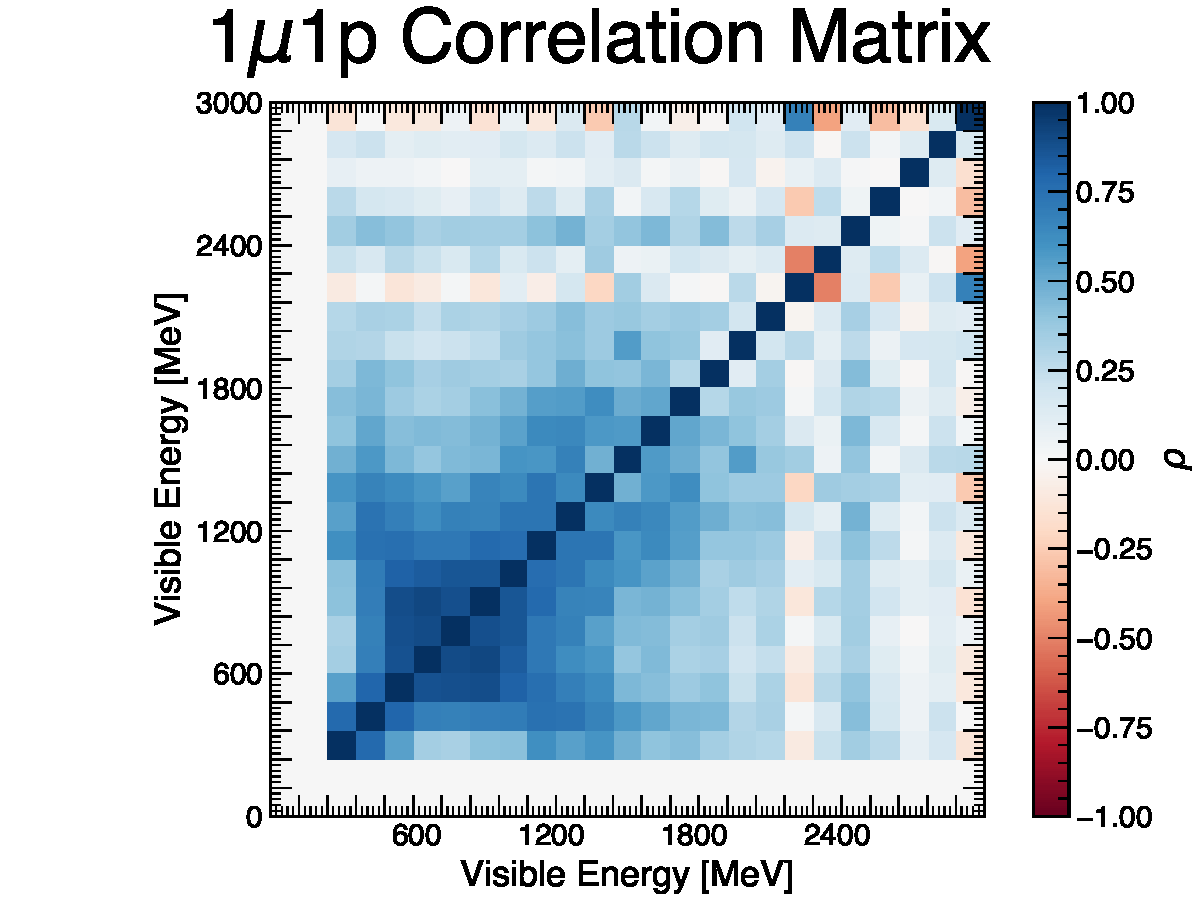
\includegraphics[width=0.55\textwidth]{figures/systematics/correlations_1mu1p.pdf} \\
    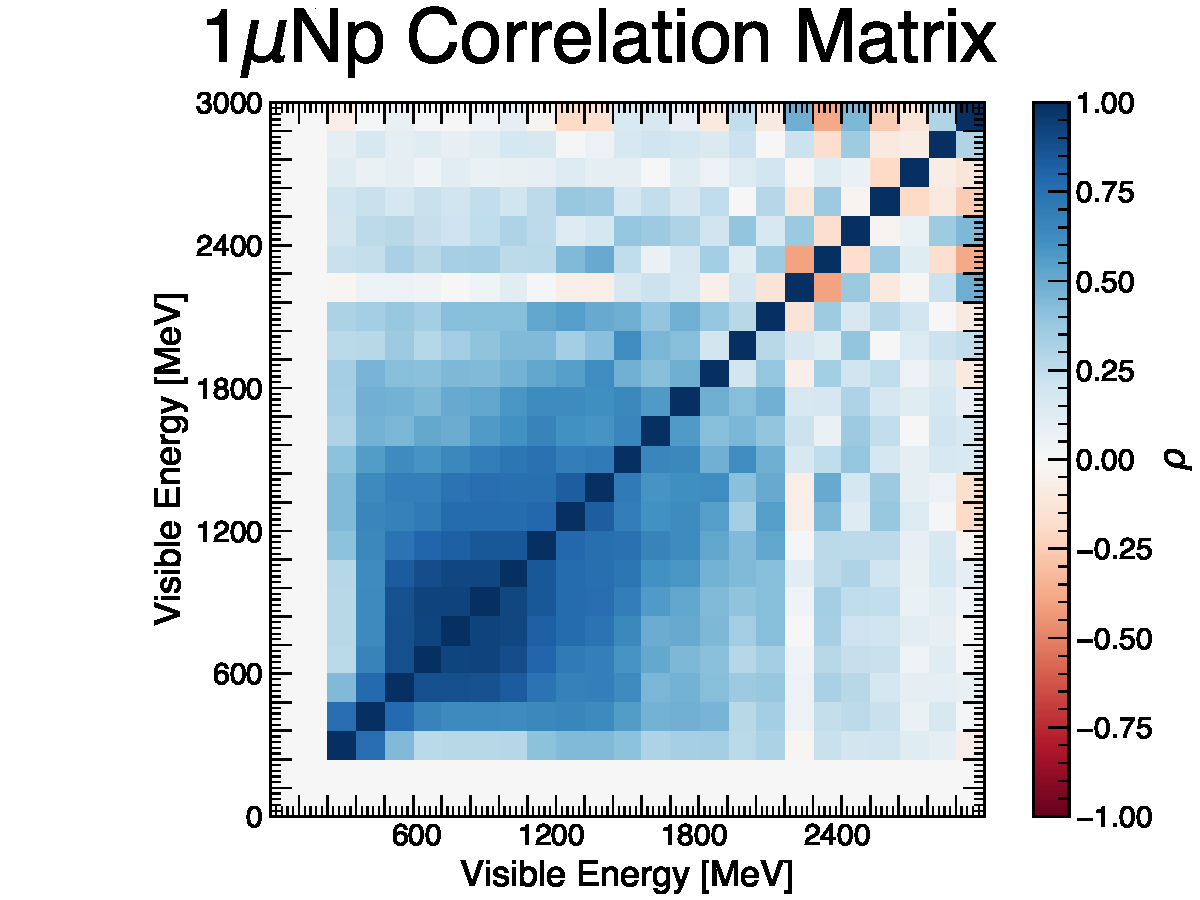
\includegraphics[width=0.55\textwidth]{figures/systematics/correlations_1muNp.pdf} \\
    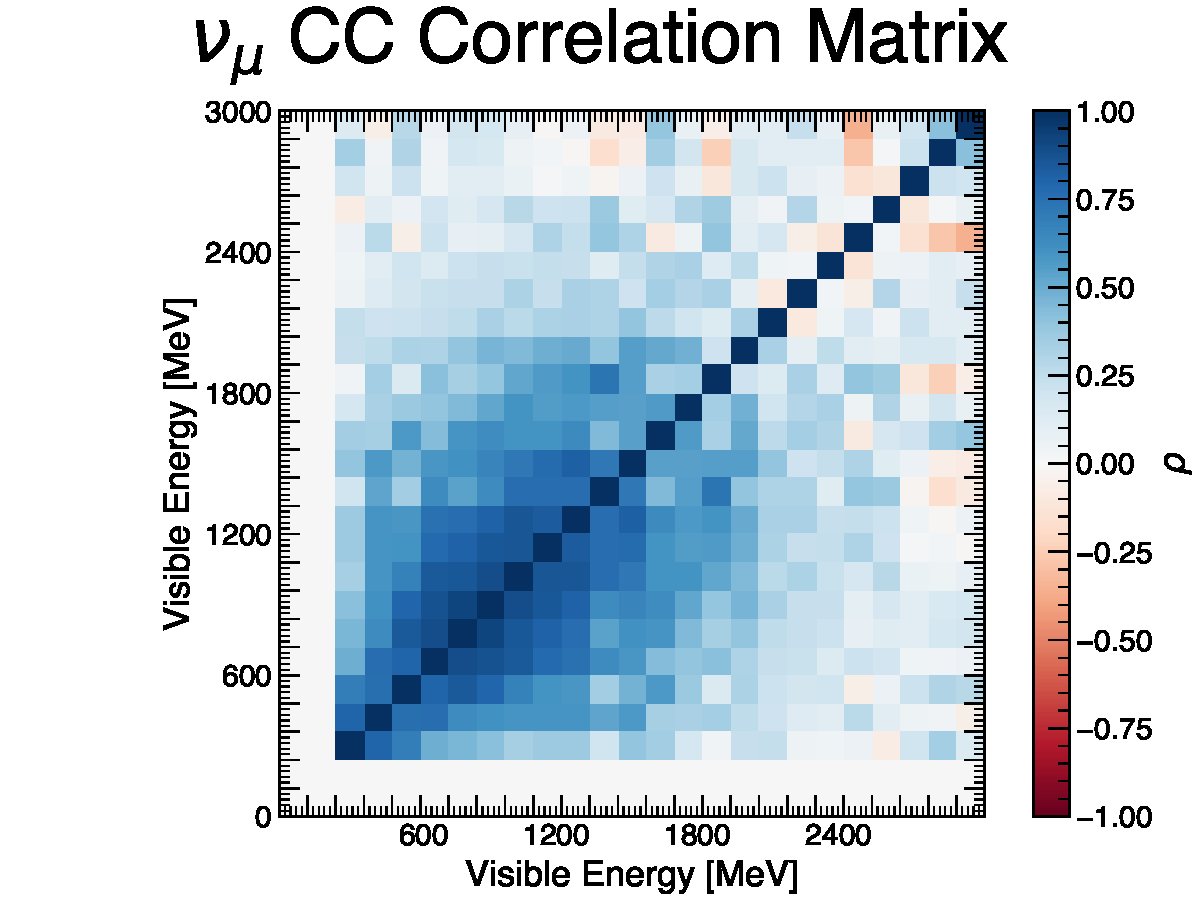
\includegraphics[width=0.55\textwidth]{figures/systematics/correlations_1muX.pdf} \\
    \caption{The total correlation matrix for the 1$\mu$1$p$ (top), 1$\mu$N$p$ (middle), and $\nu_\mu$ CC inclusive (bottom) channels. The variable shown is the reconstructed visible energy.}
    \label{fig:correlation_matrices}
\end{figure}

By far the largest source of uncertainty in the event selection is the neutrino interaction model uncertainty. This will have the biggest impact in ICARUS-only analyses, where cancellation of systematic uncertainties between the near and far detectors is not possible. The detector response uncertainty is the next largest source of uncertainty, but is expected to be reduced in future analyses as the detector response simulation is improved and more precise variations of the detector response are implemented. Looking towards joint SBN analyses where the flux and neutrino interaction model uncertainties cancel to first order, the detector response uncertainty will become the dominant source of uncertainty. The statistical uncertainty associated with the simulated central value sample and the off-beam dataset are both negligible in comparison to the other sources of uncertainty.